\documentclass[compress]{beamer}
\usepackage[
    title={Analisi prestazionale di pianificatori},
    subtitle={per un problema di Single Machine Scheduling},
    event={BnB vs Gurobi},
    author={Daniele La Prova},
    longauthor={Daniele La Prova 0320429},
    email={daniele.laprova@students.uniroma2.eu},
    institute={AMOD 2021 2022},
    longinstitute={Universita degli Studi di Roma Tor Vergata},
    department={},
    researchgroup={},
]{utvengbeamer}
\usepackage{minted}
\usepackage{amssymb}
\usepackage{mathtools}
\usepackage{dsfont}
\usepackage{hyperref}
\usepackage{scalerel}
\usepackage{datetime}
\usepackage{listings}

\useoutertheme[subsection=false]{miniframes}

\begin{document}
    
\begin{frame}[plain]
    \titlepage
    \textbf{last modified:} \today \space \currenttime \\
    \textbf{template:} \href{https://github.com/IntelligentSystemsLabUTV/UTV-Eng-beamer-template}{\texttt{utvengbeamer}}
\end{frame}

\section{Introduzione}
    \begin{frame}{\secname}
        \begin{itemize}
            \item Si vuole analizzare le prestazioni di algoritmi di pianificazione
             per un problema di Single Machine Scheduling (SMS) al variare 
             di alcune caratteristiche della sequenza di job da schedulare
             \item gli algoritmi sottoposti alla analisi sono: 
             \begin{itemize}
                \item \textbf{Branch \& Bound combinatorio:} un'implementazione che risolve
                problemi di SMS usando la regola SPTF per il calcolo dei lower bounds 
                \item \textbf{Gurobi solver:} risolutore commerciale 
             \end{itemize}
             \item I parametri prestazionali considerati per l'analisi sono:
             \begin{itemize}
                \item \textbf {tempo di esecuzione:} cronometrato con wall clock ($\Delta$ tra istante di inizio e fine esecuzione)
                \item \textbf {dimensione dell'input:} \# jobs da pianificare
            \end{itemize} 
        \end{itemize}
        \vfill
        \begin{figure}
            
\includegraphics[scale=0.5]{figs/objective.png}
            \caption{Il problema di SMS usato come Case Study}
        \end{figure}
    \end{frame}

\section{Metodologia}
    \subsection{Modellazione}
    
    \begin{frame}{\subsecname}

            \begin{itemize}
                \item Sono state fornite implementazioni degli algoritmi usando
                la tecnologia \textbf{Python}
                \item il modulo \texttt{logic.problem} definisce le seguenti interfacce:
                \begin{itemize}
                    \item \texttt{Objective}: Rappresenta il calcolo della funzione obiettivo
                    \item \texttt{Solver}: Rappresenta un algoritmo di risoluzione.
                    \item \texttt{Problem}: Rappresenta un problema generico.
                \end{itemize}
            \end{itemize}

    \end{frame}

    \begin{frame}[fragile]{\subsecname}
        \begin{itemize}
        \item Un utente puo costruire un problema instanziando una implementazione
        di \texttt{Problem} fornendogli un'istanza di implementazione di \texttt{Objective}
        e di \texttt{Solver}.
        \item Invocando il metodo \texttt{Problem.solve()} viene eseguito 
            l'algoritmo di scheduling specificato, il quale in base alla sua implementazione
            modificherà lo stato delle variabili per minimizzare o massimizzare la funzione obiettivo.    
        \end{itemize}    
                \begin{center}
                    \begin{minted}[autogobble, fontsize=\scriptsize, linenos, numbersep=3pt]{python}
                        
                        # create a problem, solve it and display the result
                        p = problem
                        p.solver = solver
                        p.objective = objective
                        p.solve()
                        print(p.value)
                    \end{minted}
                \end{center}        
    \end{frame}

    \begin{frame}{\subsecname}
        \begin{itemize}
            \item il modulo \texttt{logic.sms.entities} definisce le seguenti implementazioni
            necessarie per definire un problema di SMS:
            \begin{itemize}
                \item \texttt{Job} : Rappresenta un job con i suoi parametri, che possono essere:
                \begin{itemize}
                    \item \textbf{statici}: immutabili tra una pianificazione e l'altra (ES: processing time)
                    \item \textbf{dinamici}: possono variare tra una pianificazione e l'altra (ES: starting time)
                \end{itemize}
                \item \texttt{Machine}: Rappresenta la macchina su cui sono schedulati i job, e
                tiene traccia di parametri utili al calcolo di una pianificazioni condivisi da
                tutti i jobs (ES: un riferimento al job correntemente in esecuzione)
                \item \texttt{SingleMachineScheduling} : Una implementazione di \texttt{Problem} che
                aggrega una lista di \texttt{Job} e una \texttt{Machine}.
            \end{itemize}
        \end{itemize}
    \end{frame}

    
    \subsection{B\&B}

    \begin{frame}[fragile]{\subsecname}
        \begin{itemize}
            \item il modulo \texttt{logic.bnb} descrive l'interfaccia per un generico algoritmo
            di B\&B.
            \item Le implementazioni devono definire i seguenti metodi:
            \begin{itemize}
                \item \texttt{branch(pNode) -> list}: Implementa la generazione dei
                nodi dell albero a partire dal nodo \texttt{pNode}, se non sondato.
                Il criterio di generazione è a discrezione dell'implementazione;
                \item \texttt{isFathomed(pNode) -> bool}: Implementa i criteri di fathoming
                per decidere se un nodo è sondato o meno.
            \end{itemize}
            \item I sottoproblemi generati dalle implementazioni sono gestiti in una 
            struttura ad albero ed esplorati mediante BFS.
        \end{itemize}
    \end{frame}

    \subsection{B\&B combinatorio}
    \begin{frame}[fragile]{\subsecname}
        \begin{itemize}
            \item Il modulo \texttt{logic.sms.cbnb} descrive l'implementazione \texttt{CombinatorialBnB}
            che implementa un risolutore di problemi di SMS usando un algoritmo di B\&B.
            \item nella sua implementazione di \texttt{branch()} viene generato un sottoproblema per
            ogni istante di tempo, in modo da tenere conto della \textbf{interrompibilità} dei processi
            \begin{itemize}
                \item ogni sottoproblema è il risultato della decisione di mettere in servizio
                un diverso job, oppure di mantenere il job precedentemente in esecuzione (se possibile),
                per esattamente 1 istante di tempo
            \end{itemize}
        \end{itemize}
    \end{frame}
    \begin{frame}[fragile]{\subsecname}
        \begin{itemize}
            \item  \texttt{isFathomed()} sonda
            un sottoproblema calcolando un lower bound usando l'algoritmo passato come
            parametro al costruttore e associato al problema al momento del branching,
            applicandolo a una copia.
        \end{itemize}
        \begin{minted}[autogobble, fontsize=\scriptsize, linenos, numbersep=3pt]{python}
                                                    
            def isFathomed(self, toFathomNode):
                # a dominated problem can be immediately considered as fathomed
                if self.isDominated(toFathomNode):
                    return True
                # calculates bound on a problem copy
                toFathomCopy = deepcopy(toFathomNode.data)
                toFathomCopy.solve()  # bounding
                if toFathomCopy.value == float("nan")
                or toFathomCopy.value >= self.incumbentBound: 
                    # bound is worse than the incumbent bound,
                    # so the problem can be fathomed
                    return True
                if toFathomCopy.value < self.incumbentBound:
                    # bound is better than the incumbent bound,
                    # so the problem can be further decomposed
                    self.incumbentBound = toFathomCopy.value
                    self.incumbent = toFathomCopy.vars
                    return False
        \end{minted} 
    \end{frame}
    \begin{frame}[fragile]{\subsecname}
        \begin{itemize}
            \item La \textbf{regola di dominanza} permette di ridurre i problemi da sondare verificando
            che una pianificazione candidata rispetti le caratteristiche che una 
            pianificazione ottima deve avere.
        \end{itemize}
        \begin{theorem}[Dominance Rule]
            se il job $k$ schedulato in $pNode$ è t.c. $r_k \geq \max(r_j, t) + p_j, j$ schedulato in S, $\forall S \in sNodes \Rrightarrow $ nodo $pNode$ è sondato
        \end{theorem}
        \begin{minted}[autogobble, fontsize=\scriptsize, linenos, numbersep=3pt, numbersep=3pt]{python}
                                                    
            def isDominated(self, pNode):
                k = pNode.data.machine.currentlyScheduled        
                sNodes = self.problemsTree.siblings(pNode.identifier)
                for s in sNodes:
                    # Problem is dominated if job k is released after the estimated
                    # completion time of the currently scheduled job in all other
                    # sibling problems,assuming that no preemption occurs.
                    j = s.data.machine.currentlyScheduled
                    if k.releaseTime <= s.data.machine.currentTime + j.remainingTime:
                        return False
                return True
        \end{minted}
    \end{frame}

    \subsection{Modellazione Lineare}
    \begin{frame}{\subsecname}
        
        \begin{alignat}{4}
          & \text{min} \quad && \mathrlap{\sum_{j \in J} w_j C_j } \\ %objective
          & \text{s.t.} \quad && \sum_{j \in J} x_{jt} \leq 1 \quad && \forall t \in T \\
          & && \sum_{t \in T} x_{jt} = p_j \quad && \forall j \in J \\
          & && c_j \geq tx_{jt} \quad && \forall j \in J, t \in t \\
          & && x_{jt} \leq 0 \quad && \forall j \in J, t \leq r_j \in T\\
          & && x_{jt} \in {0, 1} \quad && \forall j \in J, t \in t\\
          & && c_j \geq 1 \in \mathds{N} \quad && \forall j \in J 
        \end{alignat}
    \end{frame}

\section{Discussione Risultati}

    \subsection{Tecnologie}
    \begin{frame}{\subsecname}
        \begin{itemize}
            \item per organizzare i dati in grafici sono stati usati i seguenti programmi:
            \begin{itemize}
                \item 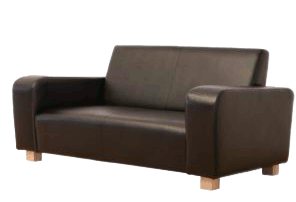
\includegraphics[scale=0.1]{figs/sofastatsLogo.png} \href{https://www.sofastatistics.com/home.php}{\textbf{SOFAstats}}:
                analizza statisticamente dati per realizzare grafici;
                \item 
\includegraphics[scale=0.1]{figs/kCacheGrindLogo-removebg-preview.png} \href{https://kcachegrind.github.io/html/Home.html}{\textbf{KCacheGrind}}: realizza mappe di chiamata 
                a funzioni a scopi di profilazione;
            \end{itemize}
            \item Il cronometraggio è stato eseguito usando la funzione \texttt{timeit} di Python,
            mentre la profilazione con la libreria \texttt{cProfile};
            \item A causa di limitazioni imposte nella licenza di Gurobi, il risolutore che lo
            implementa è limitato a un determinato \texttt{TIME\_HORIZON} di istanti di tempo
            molto inferiore a quello teorico di BnB.
            \item La generazione di parametri causali per i jobs segue una distribuzione uniforme tra
            0 e la dimensione della sequenza di jobs

        \end{itemize}
    \end{frame}
    \begin{frame}[fragile]{\subsecname}
        \begin{minted}[autogobble, fontsize=\scriptsize]{text}
            Operating System: Fedora Linux 36
            KDE Plasma Version: 5.25.5
            KDE Frameworks Version: 5.98.0
            Qt Version: 5.15.5
            Kernel Version: 5.19.11-200.fc36.x86_64 (64-bit)
            Graphics Platform: X11
            Processors: 8 × Intel® Core™ i7-4700MQ CPU @ 2.40GHz
            Memory: 15.3 GiB of RAM
            Graphics Processor: Mesa Intel® HD Graphics 4600
            Manufacturer: LENOVO
            Product Name: 20BE0087GE
            System Version: ThinkPad T540p
        \end{minted}
        \vfill
        caratteristiche macchina su cui sono stati eseguiti i test
    \end{frame}


    \subsection{Prove Sperimentali}
    \begin{frame}{\subsecname \hfill 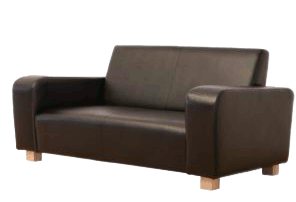
\includegraphics[scale=0.1]{figs/sofastatsLogo.png}}
        \begin{figure}
            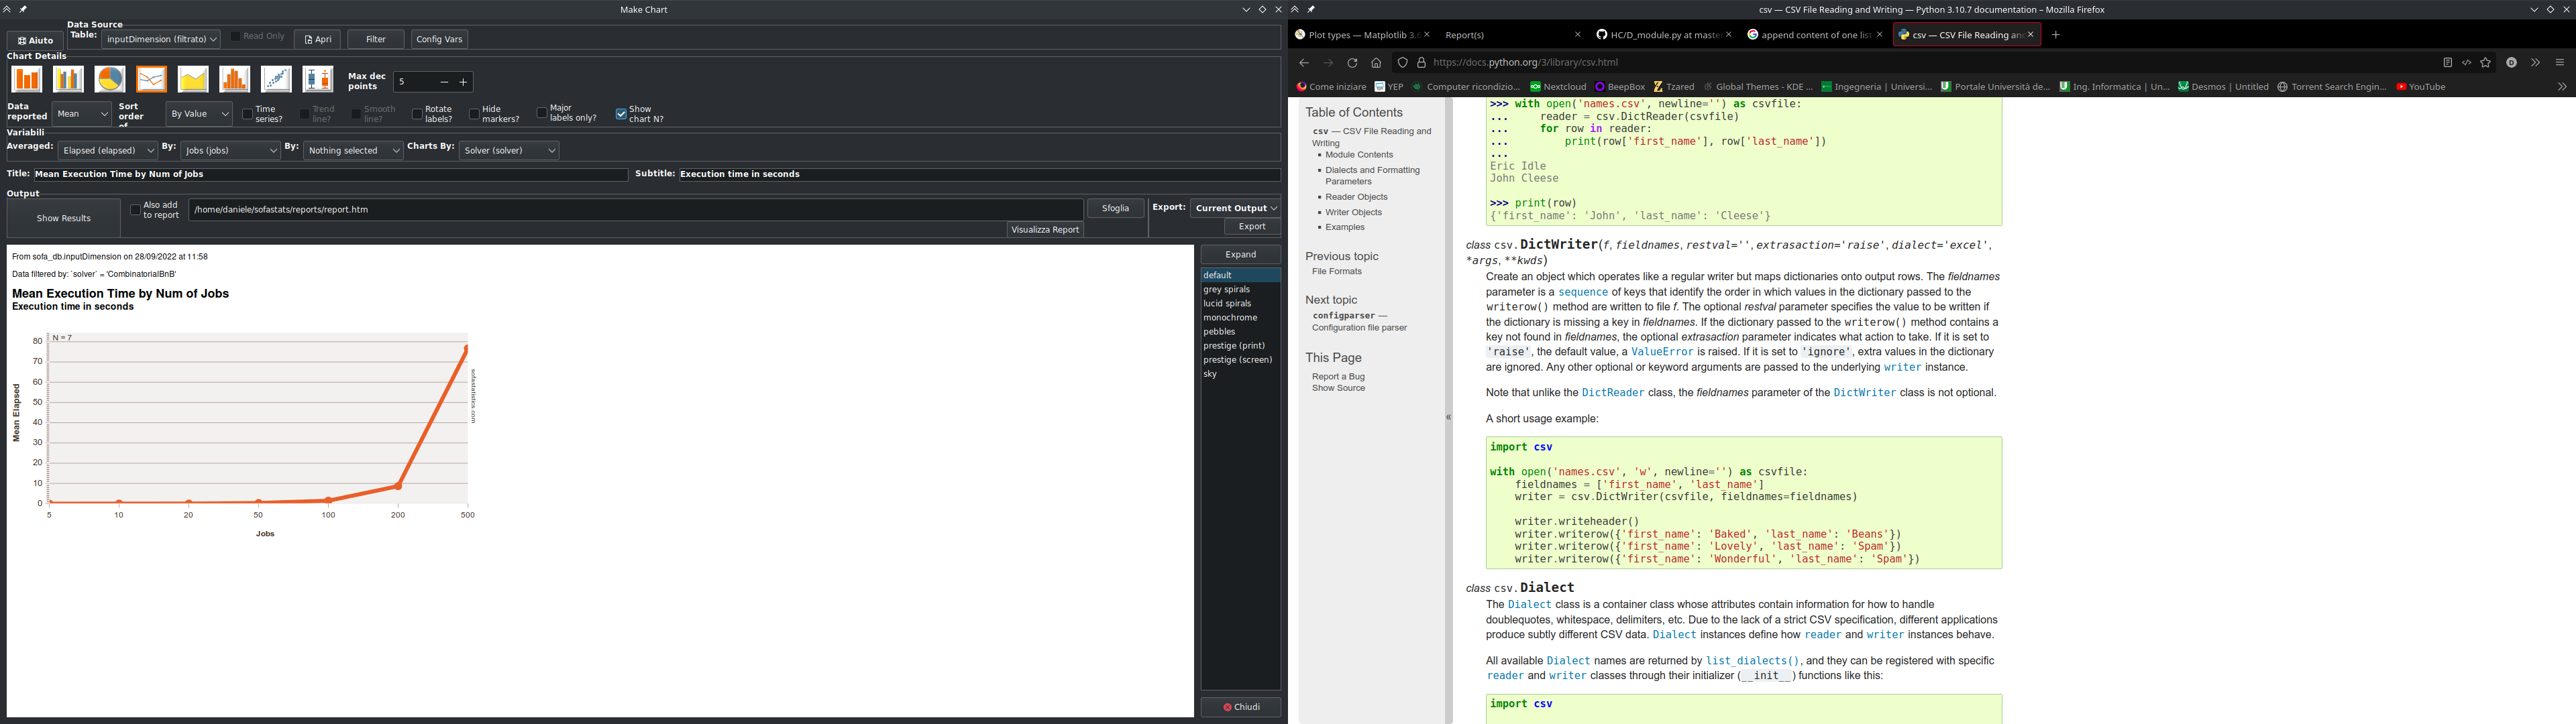
\includegraphics[scale=0.45]{../proofs/inputDimension_5-500000_meanExecByJobsBySolver_10m_lineChart.png}
            \caption[]{Tempo di esecuzione medio in funzione del numero di jobs. Ogni job 
            ha una release time pari a 0 e un peso e un processing time pari a 1. Timeout
            imposto a 10 minuti.}
            \label{fig:inputDimension_5-500000_meanExecByJobsBySolver_10m_lineChart}
        \end{figure}        
    \end{frame}
    \begin{frame}{\subsecname \hfill 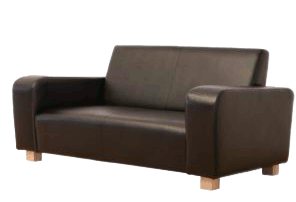
\includegraphics[scale=0.1]{figs/sofastatsLogo.png}}
        \begin{figure}
            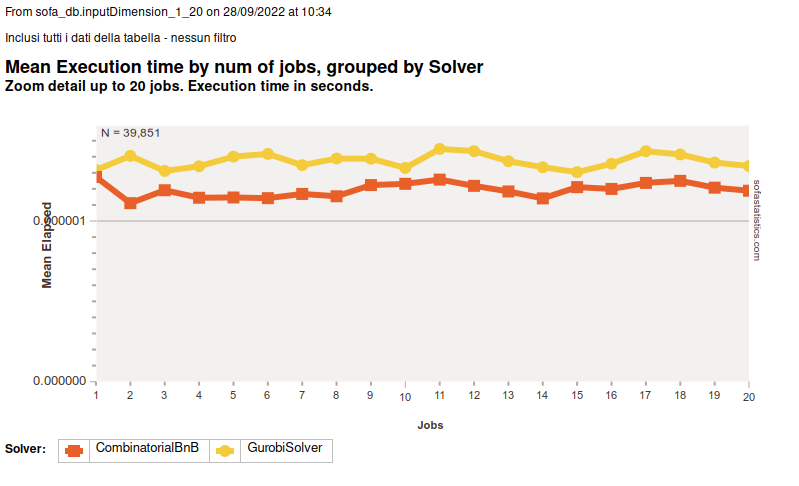
\includegraphics[scale=0.45]{../proofs/inputDimension_1-20_meanExecByJobsBySolver_lineChart.png}
            \caption[]{Zoom della figura \ref{fig:inputDimension_5-500000_meanExecByJobsBySolver_10m_lineChart}
            fino a 20 jobs.
            }
            \label{fig:inputDimension_1-20_meanExecByJobsBySolver_lineChart}
        \end{figure}        
    \end{frame}
    \begin{frame}{\subsecname \hfill 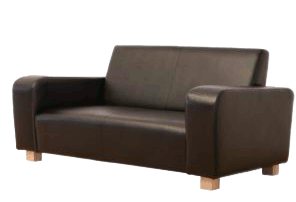
\includegraphics[scale=0.1]{figs/sofastatsLogo.png}}
        \begin{figure}
            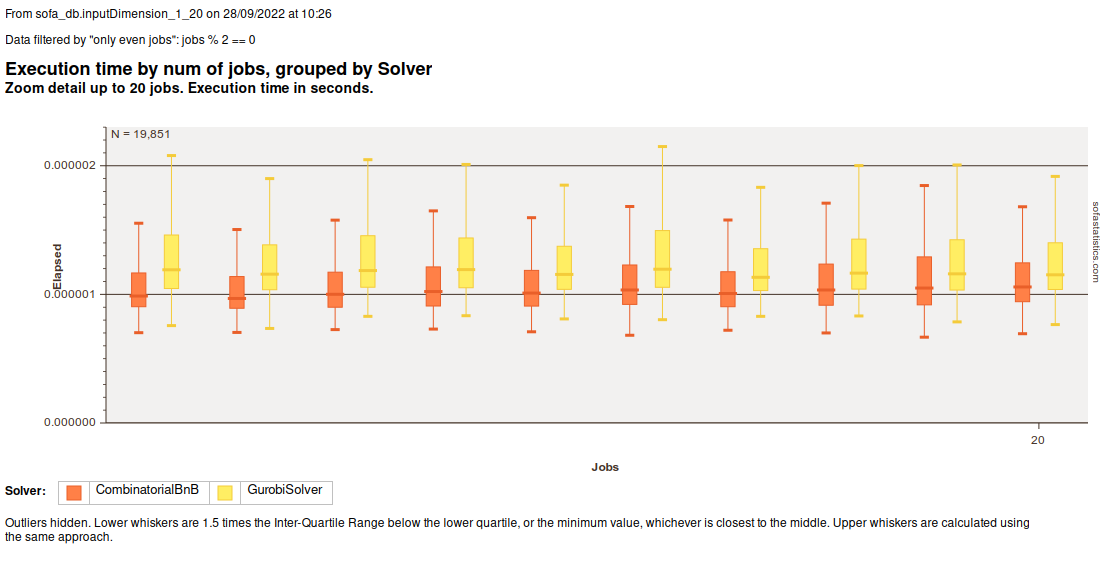
\includegraphics[scale=0.4]{../proofs/inputDimension_1-20_execByJobsBySolver_boxPlot_evenJobs.png}
            \caption[]{Vista boxplot dei tempi di esecuzione usati per calcolare le medie
            nella figura \ref{fig:inputDimension_5-500000_meanExecByJobsBySolver_10m_lineChart}.}
        \end{figure}        
    \end{frame}
    \begin{frame}{\subsecname \hfill 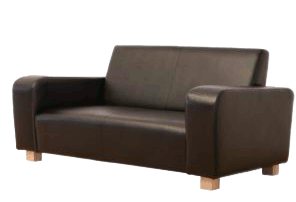
\includegraphics[scale=0.1]{figs/sofastatsLogo.png}}
        \begin{figure}
            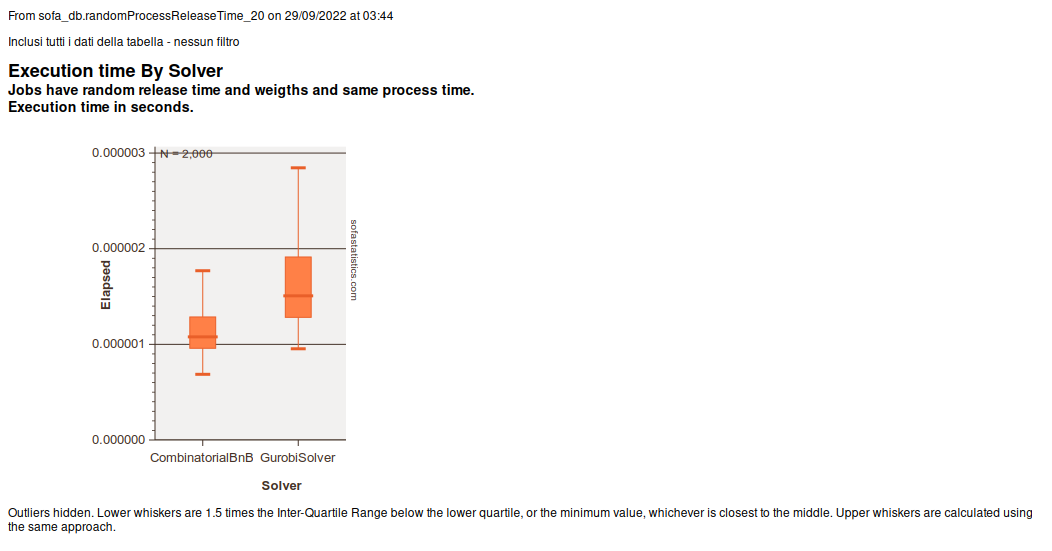
\includegraphics[scale=0.4]{../proofs/randomJobs_20_boxplot.png}
            \caption[]{Tempi di esecuzione calcolati su sequenze di 20 jobs con parametri
            casuali, ripetendo i tests per 1000 volte}
        \end{figure}        
    \end{frame}
    \begin{frame}{\subsecname \hfill 
\includegraphics[scale=0.08]{figs/kCacheGrindLogo-removebg-preview.png}}
        \begin{figure}
            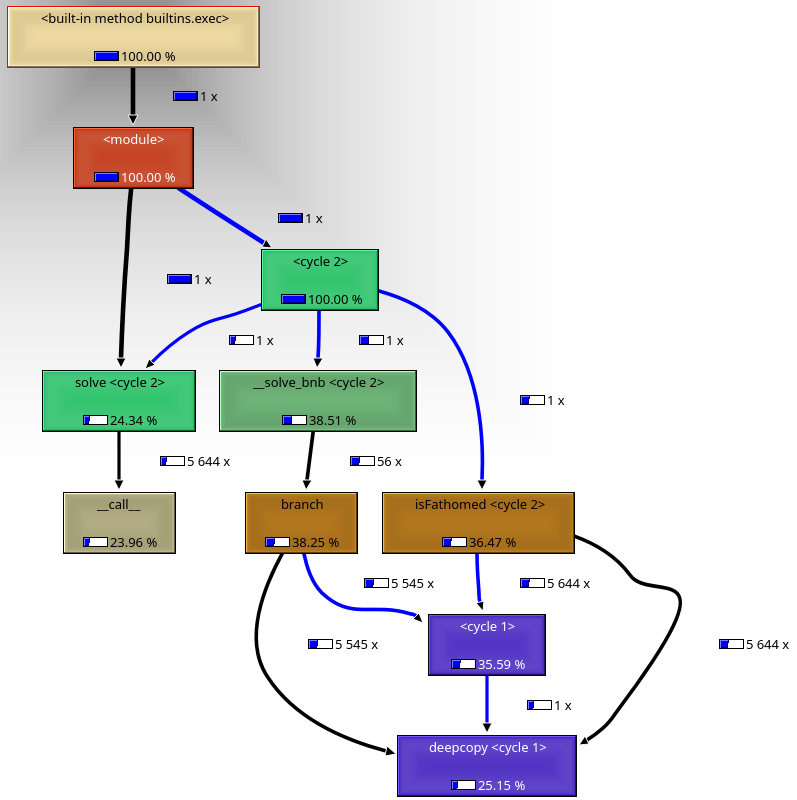
\includegraphics[scale=0.3]{../proofs/bnb_100_callstack.png}
            \caption[]{\tiny Albero delle chiamate a funzioni per BnB profilato su 100 jobs con parametri casuali.
            Le frecce in blu indicano l'appartenenza a un ciclo. Le percentuali si riferiscono
            al tempo di esecuzione dell'algoritmo.}
        \end{figure}        
    \end{frame}
\section{Conclusioni}
    \begin{frame}{\secname}
        \begin{itemize}
            \item Il risolutore B\&B risulta essere più veloce di Gurobi su sequenze
            di jobs di dimensione ridotta, sia confrontando i tempi di esecuzione medi sia quelli delle
            singole runs, sia con jobs con parametri costanti che con parametri casuali;
            \item Il tempo di esecuzione di B\&B cresce molto lentamente con il numero di jobs fino a
            circa 200 jobs, per poi crescere esponenzialmente;
            \item Le fasi di B\&B che occupano più tempo sono le chiamate a \texttt{deepcopy}
            effettuate nelle fasi di branching e fathoming (35.58\% del tempo totale). A seguire
            il calcolo del lower bound tramite SPTF (23.96\%). Lavori futuri potranno migliorare
            l'efficienza di queste fasi;

        \end{itemize}
    \end{frame}

\section{Grazie per L'attenzione!}

\begin{frame}{\secname}
    
\includegraphics[scale=0.03]{figs/GitHub-Mark.png}: \url{https://github.com/Torkin1/BnB_vs_Gurobi}
\end{frame}


\end{document}